% Options for packages loaded elsewhere
% Options for packages loaded elsewhere
\PassOptionsToPackage{unicode}{hyperref}
\PassOptionsToPackage{hyphens}{url}
\PassOptionsToPackage{dvipsnames,svgnames,x11names}{xcolor}
%
\documentclass[
  letterpaper,
  DIV=11,
  numbers=noendperiod]{scrartcl}
\usepackage{xcolor}
\usepackage{amsmath,amssymb}
\setcounter{secnumdepth}{-\maxdimen} % remove section numbering
\usepackage{iftex}
\ifPDFTeX
  \usepackage[T1]{fontenc}
  \usepackage[utf8]{inputenc}
  \usepackage{textcomp} % provide euro and other symbols
\else % if luatex or xetex
  \usepackage{unicode-math} % this also loads fontspec
  \defaultfontfeatures{Scale=MatchLowercase}
  \defaultfontfeatures[\rmfamily]{Ligatures=TeX,Scale=1}
\fi
\usepackage{lmodern}
\ifPDFTeX\else
  % xetex/luatex font selection
\fi
% Use upquote if available, for straight quotes in verbatim environments
\IfFileExists{upquote.sty}{\usepackage{upquote}}{}
\IfFileExists{microtype.sty}{% use microtype if available
  \usepackage[]{microtype}
  \UseMicrotypeSet[protrusion]{basicmath} % disable protrusion for tt fonts
}{}
\makeatletter
\@ifundefined{KOMAClassName}{% if non-KOMA class
  \IfFileExists{parskip.sty}{%
    \usepackage{parskip}
  }{% else
    \setlength{\parindent}{0pt}
    \setlength{\parskip}{6pt plus 2pt minus 1pt}}
}{% if KOMA class
  \KOMAoptions{parskip=half}}
\makeatother
% Make \paragraph and \subparagraph free-standing
\makeatletter
\ifx\paragraph\undefined\else
  \let\oldparagraph\paragraph
  \renewcommand{\paragraph}{
    \@ifstar
      \xxxParagraphStar
      \xxxParagraphNoStar
  }
  \newcommand{\xxxParagraphStar}[1]{\oldparagraph*{#1}\mbox{}}
  \newcommand{\xxxParagraphNoStar}[1]{\oldparagraph{#1}\mbox{}}
\fi
\ifx\subparagraph\undefined\else
  \let\oldsubparagraph\subparagraph
  \renewcommand{\subparagraph}{
    \@ifstar
      \xxxSubParagraphStar
      \xxxSubParagraphNoStar
  }
  \newcommand{\xxxSubParagraphStar}[1]{\oldsubparagraph*{#1}\mbox{}}
  \newcommand{\xxxSubParagraphNoStar}[1]{\oldsubparagraph{#1}\mbox{}}
\fi
\makeatother


\usepackage{longtable,booktabs,array}
\usepackage{calc} % for calculating minipage widths
% Correct order of tables after \paragraph or \subparagraph
\usepackage{etoolbox}
\makeatletter
\patchcmd\longtable{\par}{\if@noskipsec\mbox{}\fi\par}{}{}
\makeatother
% Allow footnotes in longtable head/foot
\IfFileExists{footnotehyper.sty}{\usepackage{footnotehyper}}{\usepackage{footnote}}
\makesavenoteenv{longtable}
\usepackage{graphicx}
\makeatletter
\newsavebox\pandoc@box
\newcommand*\pandocbounded[1]{% scales image to fit in text height/width
  \sbox\pandoc@box{#1}%
  \Gscale@div\@tempa{\textheight}{\dimexpr\ht\pandoc@box+\dp\pandoc@box\relax}%
  \Gscale@div\@tempb{\linewidth}{\wd\pandoc@box}%
  \ifdim\@tempb\p@<\@tempa\p@\let\@tempa\@tempb\fi% select the smaller of both
  \ifdim\@tempa\p@<\p@\scalebox{\@tempa}{\usebox\pandoc@box}%
  \else\usebox{\pandoc@box}%
  \fi%
}
% Set default figure placement to htbp
\def\fps@figure{htbp}
\makeatother





\setlength{\emergencystretch}{3em} % prevent overfull lines

\providecommand{\tightlist}{%
  \setlength{\itemsep}{0pt}\setlength{\parskip}{0pt}}



 


\KOMAoption{captions}{tableheading}
\makeatletter
\@ifpackageloaded{tcolorbox}{}{\usepackage[skins,breakable]{tcolorbox}}
\@ifpackageloaded{fontawesome5}{}{\usepackage{fontawesome5}}
\definecolor{quarto-callout-color}{HTML}{909090}
\definecolor{quarto-callout-note-color}{HTML}{0758E5}
\definecolor{quarto-callout-important-color}{HTML}{CC1914}
\definecolor{quarto-callout-warning-color}{HTML}{EB9113}
\definecolor{quarto-callout-tip-color}{HTML}{00A047}
\definecolor{quarto-callout-caution-color}{HTML}{FC5300}
\definecolor{quarto-callout-color-frame}{HTML}{acacac}
\definecolor{quarto-callout-note-color-frame}{HTML}{4582ec}
\definecolor{quarto-callout-important-color-frame}{HTML}{d9534f}
\definecolor{quarto-callout-warning-color-frame}{HTML}{f0ad4e}
\definecolor{quarto-callout-tip-color-frame}{HTML}{02b875}
\definecolor{quarto-callout-caution-color-frame}{HTML}{fd7e14}
\makeatother
\makeatletter
\@ifpackageloaded{caption}{}{\usepackage{caption}}
\AtBeginDocument{%
\ifdefined\contentsname
  \renewcommand*\contentsname{Table of contents}
\else
  \newcommand\contentsname{Table of contents}
\fi
\ifdefined\listfigurename
  \renewcommand*\listfigurename{List of Figures}
\else
  \newcommand\listfigurename{List of Figures}
\fi
\ifdefined\listtablename
  \renewcommand*\listtablename{List of Tables}
\else
  \newcommand\listtablename{List of Tables}
\fi
\ifdefined\figurename
  \renewcommand*\figurename{Figure}
\else
  \newcommand\figurename{Figure}
\fi
\ifdefined\tablename
  \renewcommand*\tablename{Table}
\else
  \newcommand\tablename{Table}
\fi
}
\@ifpackageloaded{float}{}{\usepackage{float}}
\floatstyle{ruled}
\@ifundefined{c@chapter}{\newfloat{codelisting}{h}{lop}}{\newfloat{codelisting}{h}{lop}[chapter]}
\floatname{codelisting}{Listing}
\newcommand*\listoflistings{\listof{codelisting}{List of Listings}}
\makeatother
\makeatletter
\makeatother
\makeatletter
\@ifpackageloaded{caption}{}{\usepackage{caption}}
\@ifpackageloaded{subcaption}{}{\usepackage{subcaption}}
\makeatother
\usepackage{bookmark}
\IfFileExists{xurl.sty}{\usepackage{xurl}}{} % add URL line breaks if available
\urlstyle{same}
\hypersetup{
  pdftitle={ BANA 4080},
  colorlinks=true,
  linkcolor={blue},
  filecolor={Maroon},
  citecolor={Blue},
  urlcolor={Blue},
  pdfcreator={LaTeX via pandoc}}


\title{BANA 4080}
\author{}
\date{}
\begin{document}
\maketitle


\section{Welcome to BANA 4080}\label{welcome-to-bana-4080}

\subsection{Brad Boehmke}\label{brad-boehmke}

\begin{itemize}
\item
  Phonetically: \textbf{``Bem''} + \textbf{``Key''}
\item
  Alternatives:

  \begin{itemize}
  \tightlist
  \item
    Dr.~/ Professor B
  \item
    Brad
  \end{itemize}
\item
  Contact:

  \begin{itemize}
  \tightlist
  \item
    Read \textbf{Communication Expectations} Canvas page first!
  \item
    Email: boehmkbc@ucmail.uc.edu
  \item
    Office: Lindhall 3412
  \end{itemize}
\end{itemize}

\pandocbounded{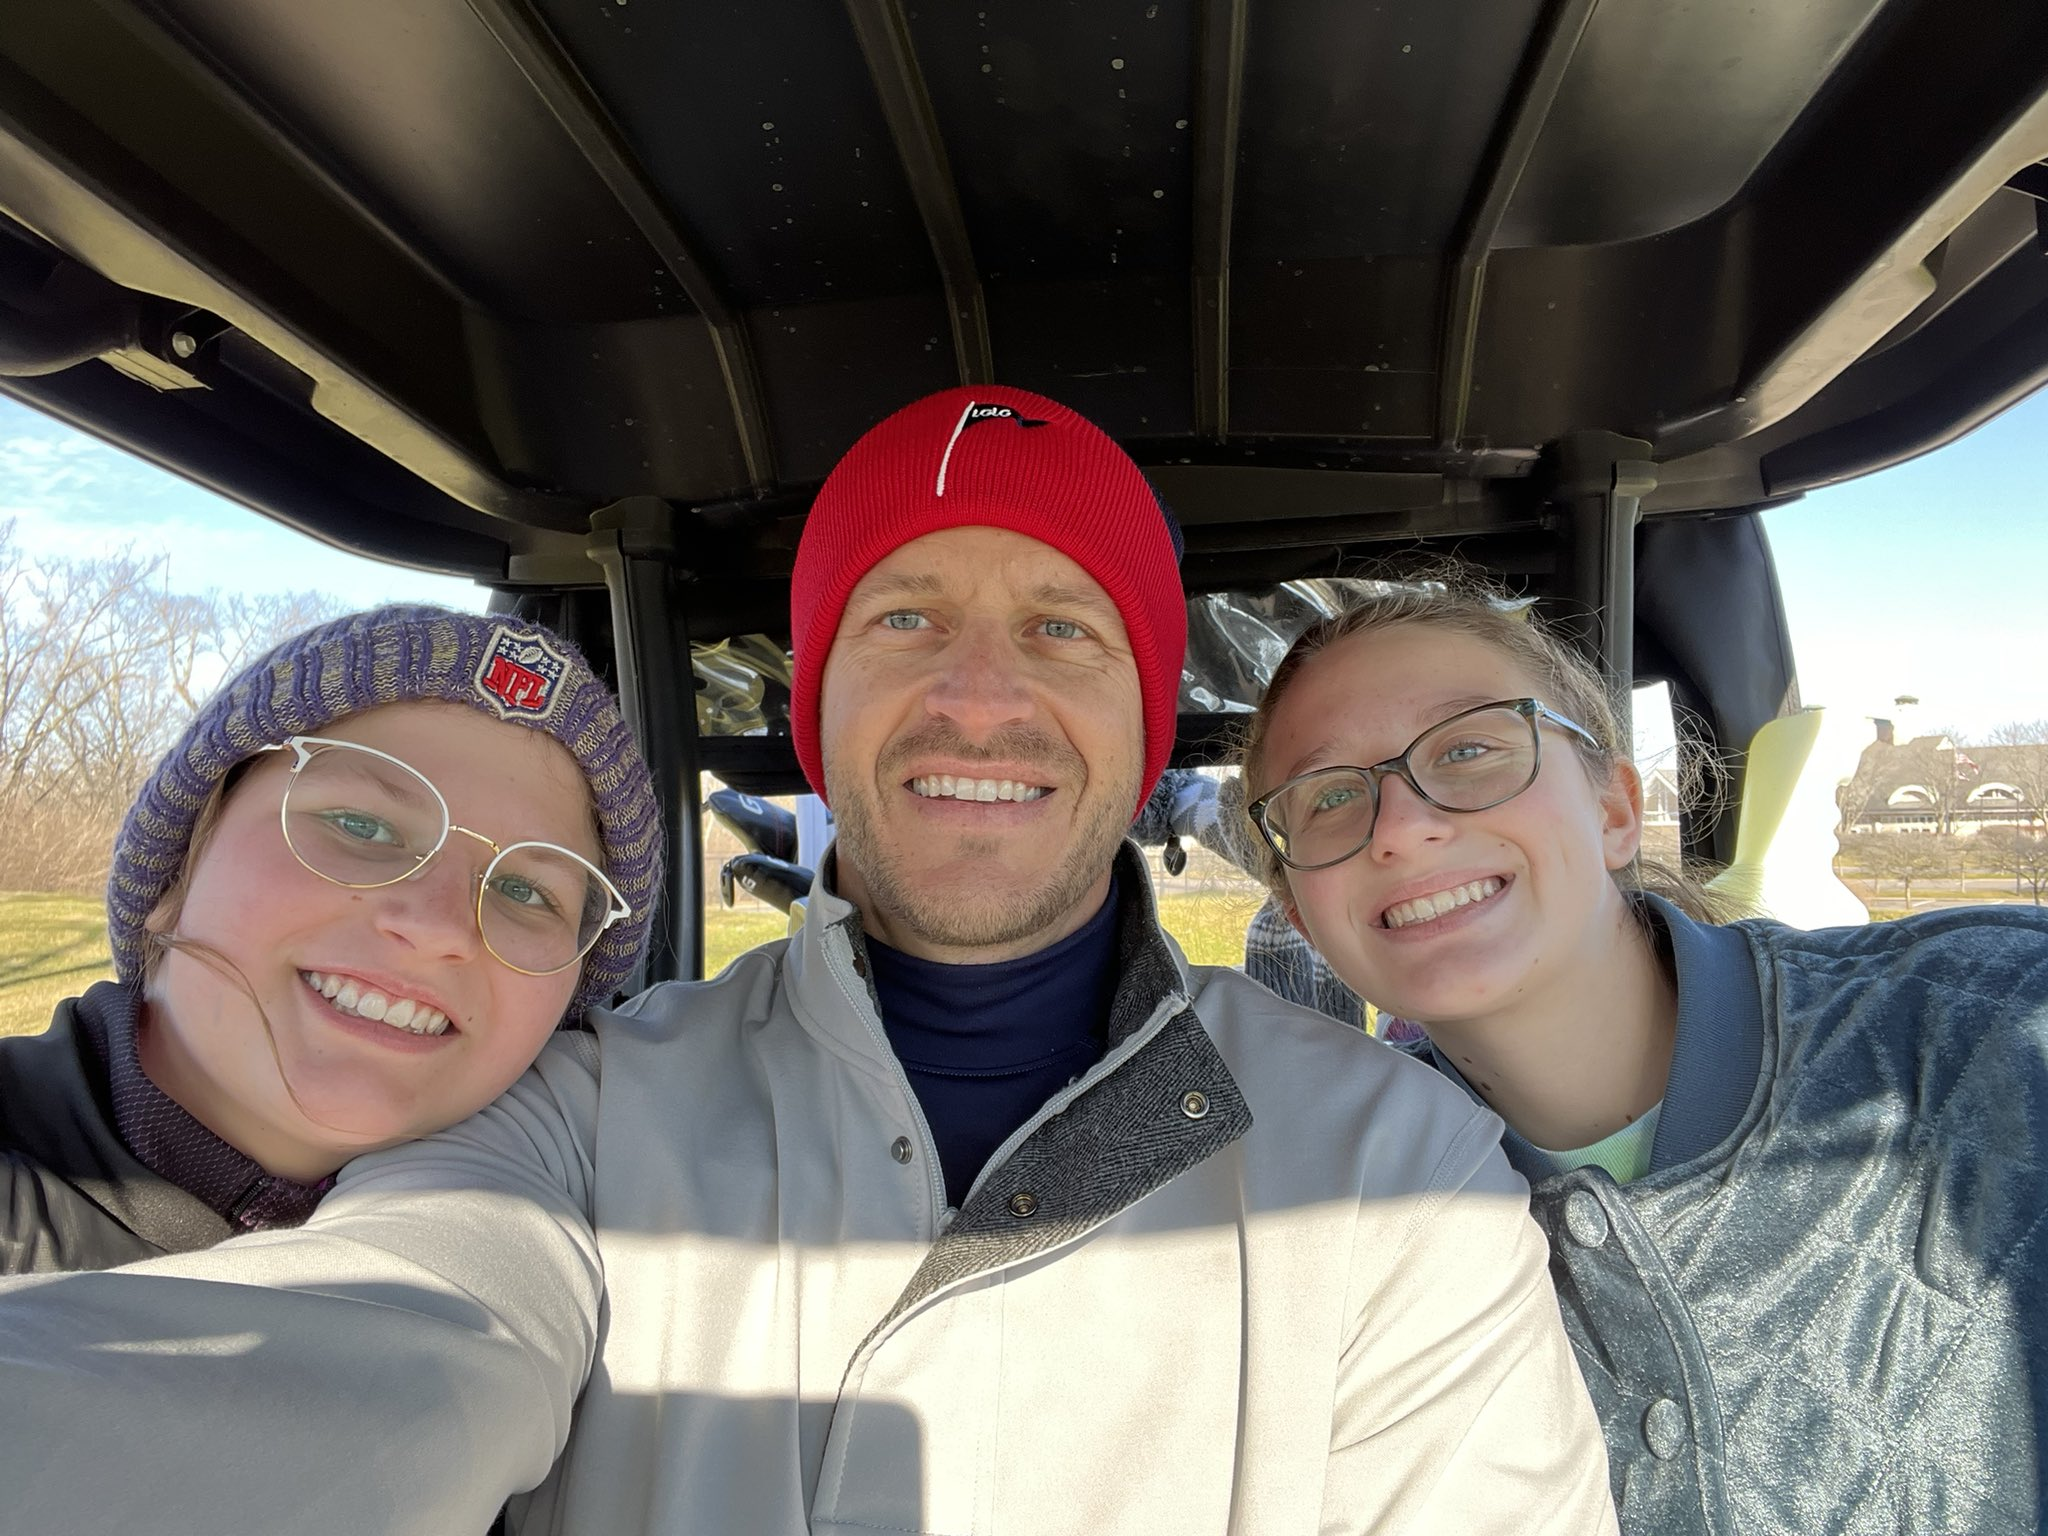
\includegraphics[keepaspectratio]{images/me.jpeg}}

\begin{center}\rule{0.5\linewidth}{0.5pt}\end{center}

\begin{center}
\pandocbounded{
\includegraphics[keepaspectratio]{images/UC.png}}
\end{center}

\pandocbounded{
\includegraphics[keepaspectratio]{images/8451.jpg}}\hfill

\begin{center}
\pandocbounded{
\includegraphics[keepaspectratio]{images/kroger.png}}
\end{center}

\begin{center}\rule{0.5\linewidth}{0.5pt}\end{center}

\subsection{Fun Fact: Golf Obsessed}\label{fun-fact-golf-obsessed}

\subsection{Meet Your TA}\label{meet-your-ta}

\subsubsection{👋 {[}TA Name{]}}\label{ta-name}

\begin{itemize}
\tightlist
\item
  {[}Junior/Senior/Graduate student{]} in Business Analytics\\
\item
  Passionate about helping you succeed\\
\item
  Great resource for coding questions, labs, and homework
\end{itemize}

📧 Email: {[}TA Email{]}\\
🕐 Office Hours: {[}Insert schedule or by appointment{]}

\begin{tcolorbox}[enhanced jigsaw, colbacktitle=quarto-callout-important-color!10!white, opacityback=0, colback=white, opacitybacktitle=0.6, toptitle=1mm, left=2mm, bottomrule=.15mm, breakable, bottomtitle=1mm, rightrule=.15mm, titlerule=0mm, title=\textcolor{quarto-callout-important-color}{\faExclamation}\hspace{0.5em}{Important}, coltitle=black, colframe=quarto-callout-important-color-frame, arc=.35mm, toprule=.15mm, leftrule=.75mm]

Don't hesitate to reach out --- they're here to support you!

\end{tcolorbox}

\subsection{Today's Agenda}\label{todays-agenda}

\begin{itemize}
\tightlist
\item
  What is data mining?
\item
  Course overview \& goals
\item
  Course roadmap
\item
  Tools \& setup preview
\item
  Why Python?
\item
  Q\&A + student discussion
\end{itemize}

\section{What is Data Mining}\label{what-is-data-mining}

\subsection{Data Mining is All Around
Us}\label{data-mining-is-all-around-us}

\begin{quote}
Organizations use data mining to drive decisions every day.
\end{quote}

\textbf{Real-World Examples:}

\begin{itemize}
\tightlist
\item
  🛒 \emph{Kroger analyzes loyalty card data} to personalize digital
  coupons.
\item
  🎶 \emph{Spotify recommends music} based on your listening history and
  those like you.
\item
  🏥 \emph{Hospitals use patient data} to predict readmission risks.
\item
  🏈 \emph{NFL teams analyze player movement data} to improve
  performance and strategy.
\item
  📦 \emph{Amazon tracks browsing behavior} to recommend products and
  optimize inventory.
\end{itemize}

. . .

\begin{tcolorbox}[enhanced jigsaw, colbacktitle=quarto-callout-important-color!10!white, opacityback=0, colback=white, opacitybacktitle=0.6, toptitle=1mm, left=2mm, bottomrule=.15mm, breakable, bottomtitle=1mm, rightrule=.15mm, titlerule=0mm, title=\textcolor{quarto-callout-important-color}{\faExclamation}\hspace{0.5em}{Important}, coltitle=black, colframe=quarto-callout-important-color-frame, arc=.35mm, toprule=.15mm, leftrule=.75mm]

{Every time you browse, click, buy, swipe, or stream --- you're
generating data.}

\end{tcolorbox}

\subsection{What Is Data Mining?}\label{what-is-data-mining-1}

\begin{quote}
\textbf{The process of uncovering meaningful patterns, trends, and
relationships in large data sets}
\end{quote}

Why is it important?

\begin{itemize}
\tightlist
\item
  📈 Helps organizations \textbf{make better decisions}
\item
  🔍 Reveals insights that would otherwise go unnoticed
\item
  🤖 Powers personalization, prediction, and automation
\item
  💰 Drives business value in nearly every industry
\end{itemize}

. . .

\begin{tcolorbox}[enhanced jigsaw, colbacktitle=quarto-callout-important-color!10!white, opacityback=0, colback=white, opacitybacktitle=0.6, toptitle=1mm, left=2mm, bottomrule=.15mm, breakable, bottomtitle=1mm, rightrule=.15mm, titlerule=0mm, title=\textcolor{quarto-callout-important-color}{\faExclamation}\hspace{0.5em}{Important}, coltitle=black, colframe=quarto-callout-important-color-frame, arc=.35mm, toprule=.15mm, leftrule=.75mm]

{Data mining turns raw information into \textbf{actionable knowledge}}

\end{tcolorbox}

\subsection{Activity}\label{activity}

\begin{tcolorbox}[enhanced jigsaw, leftrule=.75mm, opacityback=0, colback=white, breakable, toprule=.15mm, rightrule=.15mm, left=2mm, colframe=quarto-callout-color-frame, arc=.35mm, bottomrule=.15mm]

\vspace{-3mm}\textbf{Where Do You See Data Mining?}\vspace{3mm}

🤔 Think about your daily routine --- when are you being ``mined''?

\end{tcolorbox}

. . .

\paragraph{Instructions:}\label{instructions}

\begin{enumerate}
\def\labelenumi{\arabic{enumi}.}
\tightlist
\item
  \textbf{Form groups of 2--3 students}
\item
  Brainstorm at least \textbf{3 examples} where you think data mining is
  happening in your life
\item
  We'll share a few examples as a class
\end{enumerate}

💬 Look for clues in:

\begin{itemize}
\tightlist
\item
  Shopping \& entertainment
\item
  Health \& fitness
\item
  Social media \& tech
\item
  Education or travel
\end{itemize}

Please think about this for 5 minutes.

\phantomsection\label{5minWaiting}

\section{Challenge}\label{challenge}

\subsection{In-Class Challenge: Your First Day on the
Job}\label{in-class-challenge-your-first-day-on-the-job}

🎉 You just landed your first internship or job at a large retail
company. On Day 1, your manager says:

\begin{quote}
``We're trying to understand what drives repeat purchases. Can you dig
into this and see what you find?''
\end{quote}

You've been handed three datasets:

\begin{itemize}
\tightlist
\item
  🧾 \textbf{Customer Transactions}
\item
  🛒 \textbf{Product Information}
\item
  👥 \textbf{Customer Demographics}
\end{itemize}

Download the data from

\url{https://tinyurl.com/retail-data}

\begin{tcolorbox}[enhanced jigsaw, leftrule=.75mm, opacityback=0, colback=white, breakable, toprule=.15mm, rightrule=.15mm, left=2mm, colframe=quarto-callout-color-frame, arc=.35mm, bottomrule=.15mm]

What do you do next?

\end{tcolorbox}

\subsection{Group Activity: Where Would You
Start?}\label{group-activity-where-would-you-start}

Work in groups of 2--3 and discuss:

\begin{itemize}
\tightlist
\item
  🤔 What kinds of questions could you ask?
\item
  🔍 What would you look for in the data?
\item
  🛠️ What tools or skills do you wish you had?
\item
  💬 What's hard about this kind of open-ended problem?
\end{itemize}

Please think about this for 8 minutes.

\phantomsection\label{8minWaiting}

\begin{tcolorbox}[enhanced jigsaw, colbacktitle=quarto-callout-important-color!10!white, opacityback=0, colback=white, opacitybacktitle=0.6, toptitle=1mm, left=2mm, bottomrule=.15mm, breakable, bottomtitle=1mm, rightrule=.15mm, titlerule=0mm, title=\textcolor{quarto-callout-important-color}{\faExclamation}\hspace{0.5em}{Important}, coltitle=black, colframe=quarto-callout-important-color-frame, arc=.35mm, toprule=.15mm, leftrule=.75mm]

There's no ``right answer'' --- this is what real-world analysis looks
like.

\end{tcolorbox}

\subsection{Debrief: What Did You
Learn?}\label{debrief-what-did-you-learn}

Let's talk through what made this challenge\ldots{} challenging:

\begin{itemize}
\tightlist
\item
  🧭 How did it feel to be given a \textbf{vague problem}?
\item
  📊 What did you want to know about the data before starting?
\item
  🧠 What tools or skills do you wish you had?
\item
  💬 Did your group take different approaches?
\end{itemize}

\subsubsection{Key Takeaways:}\label{key-takeaways}

\begin{itemize}
\tightlist
\item
  Real-world problems rarely come with clean instructions
\item
  Good data work starts with \textbf{asking the right questions}
\item
  This course will help you learn how to \textbf{explore},
  \textbf{analyze}, and \textbf{communicate} insights from messy data
\end{itemize}

\section{Course Overview}\label{course-overview}

\subsection{Why Learn Data Mining?}\label{why-learn-data-mining}

Data is everywhere --- but insight is rare.

\textbf{Regardless of your major, data mining gives you a competitive
edge:}

\begin{itemize}
\tightlist
\item
  📊 \textbf{Marketing:} Understand customer behavior and optimize
  campaigns
\item
  💵 \textbf{Finance:} Detect fraud, model risk, and forecast
  performance
\item
  🏭 \textbf{Operations:} Improve efficiency, forecast demand, reduce
  waste
\item
  👩‍💼 \textbf{Management:} Support evidence-based decisions across teams
\end{itemize}

\begin{tcolorbox}[enhanced jigsaw, colbacktitle=quarto-callout-important-color!10!white, opacityback=0, colback=white, opacitybacktitle=0.6, toptitle=1mm, left=2mm, bottomrule=.15mm, breakable, bottomtitle=1mm, rightrule=.15mm, titlerule=0mm, title=\textcolor{quarto-callout-important-color}{\faExclamation}\hspace{0.5em}{Important}, coltitle=black, colframe=quarto-callout-important-color-frame, arc=.35mm, toprule=.15mm, leftrule=.75mm]

{Today's business leaders are expected to be \textbf{data-savvy decision
makers}}

\end{tcolorbox}

\subsection{What You'll Learn in BANA
4080}\label{what-youll-learn-in-bana-4080}

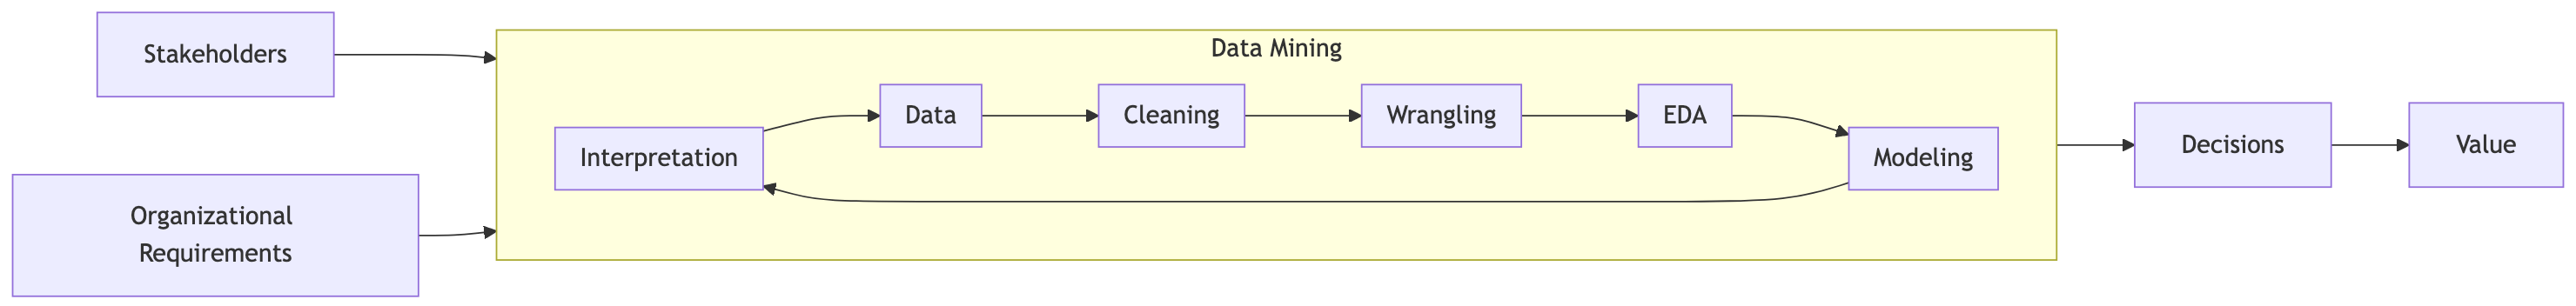
\includegraphics[width=17.19in,height=2.06in]{w1_tuesday_intro_files/figure-latex/mermaid-figure-1.png}

By the end of this course, you'll be able to:

\begin{itemize}
\tightlist
\item
  Write basic Python code to work with data
\item
  Clean, wrangle, and analyze messy real-world datasets
\item
  Visualize insights clearly and effectively
\item
  Understand how various ML/AI models are used in organizations
\item
  Build simple ML/AI models for prediction and pattern discovery
\item
  Communicate data-driven findings to others
\end{itemize}

. . .

\begin{tcolorbox}[enhanced jigsaw, colbacktitle=quarto-callout-important-color!10!white, opacityback=0, colback=white, opacitybacktitle=0.6, toptitle=1mm, left=2mm, bottomrule=.15mm, breakable, bottomtitle=1mm, rightrule=.15mm, titlerule=0mm, title=\textcolor{quarto-callout-important-color}{\faExclamation}\hspace{0.5em}{Important}, coltitle=black, colframe=quarto-callout-important-color-frame, arc=.35mm, toprule=.15mm, leftrule=.75mm]

{This course is not about memorizing syntax --- it's about
\textbf{thinking with data}}

\end{tcolorbox}

\subsection{What About AI? Won't It Do This for
Me?}\label{what-about-ai-wont-it-do-this-for-me}

🤖 AI tools like ChatGPT are amazing --- but they don't replace
\textbf{thinking with data}.

\begin{itemize}
\tightlist
\item
  AI can help you write code\ldots{} but it won't \textbf{ask the right
  questions}
\item
  AI can summarize data\ldots{} but it can't \textbf{understand your
  business context}
\item
  AI is only as good as the \textbf{data, prompts, and interpretation}
  you provide
\end{itemize}

\begin{center}
\pandocbounded{\includegraphics[keepaspectratio]{images/let-chatgpt-do-it.gif}}
\end{center}

\begin{tcolorbox}[enhanced jigsaw, colbacktitle=quarto-callout-important-color!10!white, opacityback=0, colback=white, opacitybacktitle=0.6, toptitle=1mm, left=2mm, bottomrule=.15mm, breakable, bottomtitle=1mm, rightrule=.15mm, titlerule=0mm, title=\textcolor{quarto-callout-important-color}{\faExclamation}\hspace{0.5em}{Important}, coltitle=black, colframe=quarto-callout-important-color-frame, arc=.35mm, toprule=.15mm, leftrule=.75mm]

{The future belongs to people who know how to \textbf{collaborate with
AI}, not be replaced by it. You will learn to use AI to help you build
solutions.}

\end{tcolorbox}

\section{Course Roadmap}\label{course-roadmap}

\subsection{Course Roadmap}\label{course-roadmap-1}

Your journey through BANA 4080:

\begin{enumerate}
\def\labelenumi{\arabic{enumi}.}
\tightlist
\item
  \textbf{Weeks 1--3}: Python basics \& Working with data
\item
  \textbf{Weeks 3--4}: Data wrangling \& Exploratory analysis
\item
  \textbf{Weeks 5-6}: Data visualization \& Efficient programming
\item
  \textbf{Week 7}: Mid-term
\item
  \textbf{Weeks 8-12}: ML \& AI
\item
  \textbf{Weeks 13-14}: Final project
\end{enumerate}

\begin{tcolorbox}[enhanced jigsaw, colbacktitle=quarto-callout-important-color!10!white, opacityback=0, colback=white, opacitybacktitle=0.6, toptitle=1mm, left=2mm, bottomrule=.15mm, breakable, bottomtitle=1mm, rightrule=.15mm, titlerule=0mm, title=\textcolor{quarto-callout-important-color}{\faExclamation}\hspace{0.5em}{Important}, coltitle=black, colframe=quarto-callout-important-color-frame, arc=.35mm, toprule=.15mm, leftrule=.75mm]

{This course builds your skills step-by-step --- like a training plan
for thinking with data.}

\end{tcolorbox}

\subsection{How You'll Learn}\label{how-youll-learn}

Each week follows a consistent rhythm:

\begin{itemize}
\tightlist
\item
  🧠 \textbf{Tuesday (Lecture):} Learn concepts, explore examples,
  discuss ideas
\item
  💻 \textbf{Thursday (Lab):} Practice coding, get hands-on, work with
  real data
\end{itemize}

Assessments include:

\begin{itemize}
\tightlist
\item
  📚 Weekly reading quizzes\\
\item
  📝 Biweekly homework assignments\\
\item
  📊 Midterm and final project\\
\item
  ❌ No conventional tests!
\end{itemize}

\begin{tcolorbox}[enhanced jigsaw, colbacktitle=quarto-callout-important-color!10!white, opacityback=0, colback=white, opacitybacktitle=0.6, toptitle=1mm, left=2mm, bottomrule=.15mm, breakable, bottomtitle=1mm, rightrule=.15mm, titlerule=0mm, title=\textcolor{quarto-callout-important-color}{\faExclamation}\hspace{0.5em}{Important}, coltitle=black, colframe=quarto-callout-important-color-frame, arc=.35mm, toprule=.15mm, leftrule=.75mm]

{Expect to build something meaningful --- not just learn theory.}

\end{tcolorbox}

\subsection{Resources}\label{resources}

Everything You Need Is in One of Two Spots

\paragraph{📍 Course Canvas Page}\label{course-canvas-page}

\begin{center}
\pandocbounded{
\includegraphics[keepaspectratio]{images/canvas_screenshot.png}}
\end{center}

\paragraph{📘 Course Textbook}\label{course-textbook}

\begin{center}
\pandocbounded{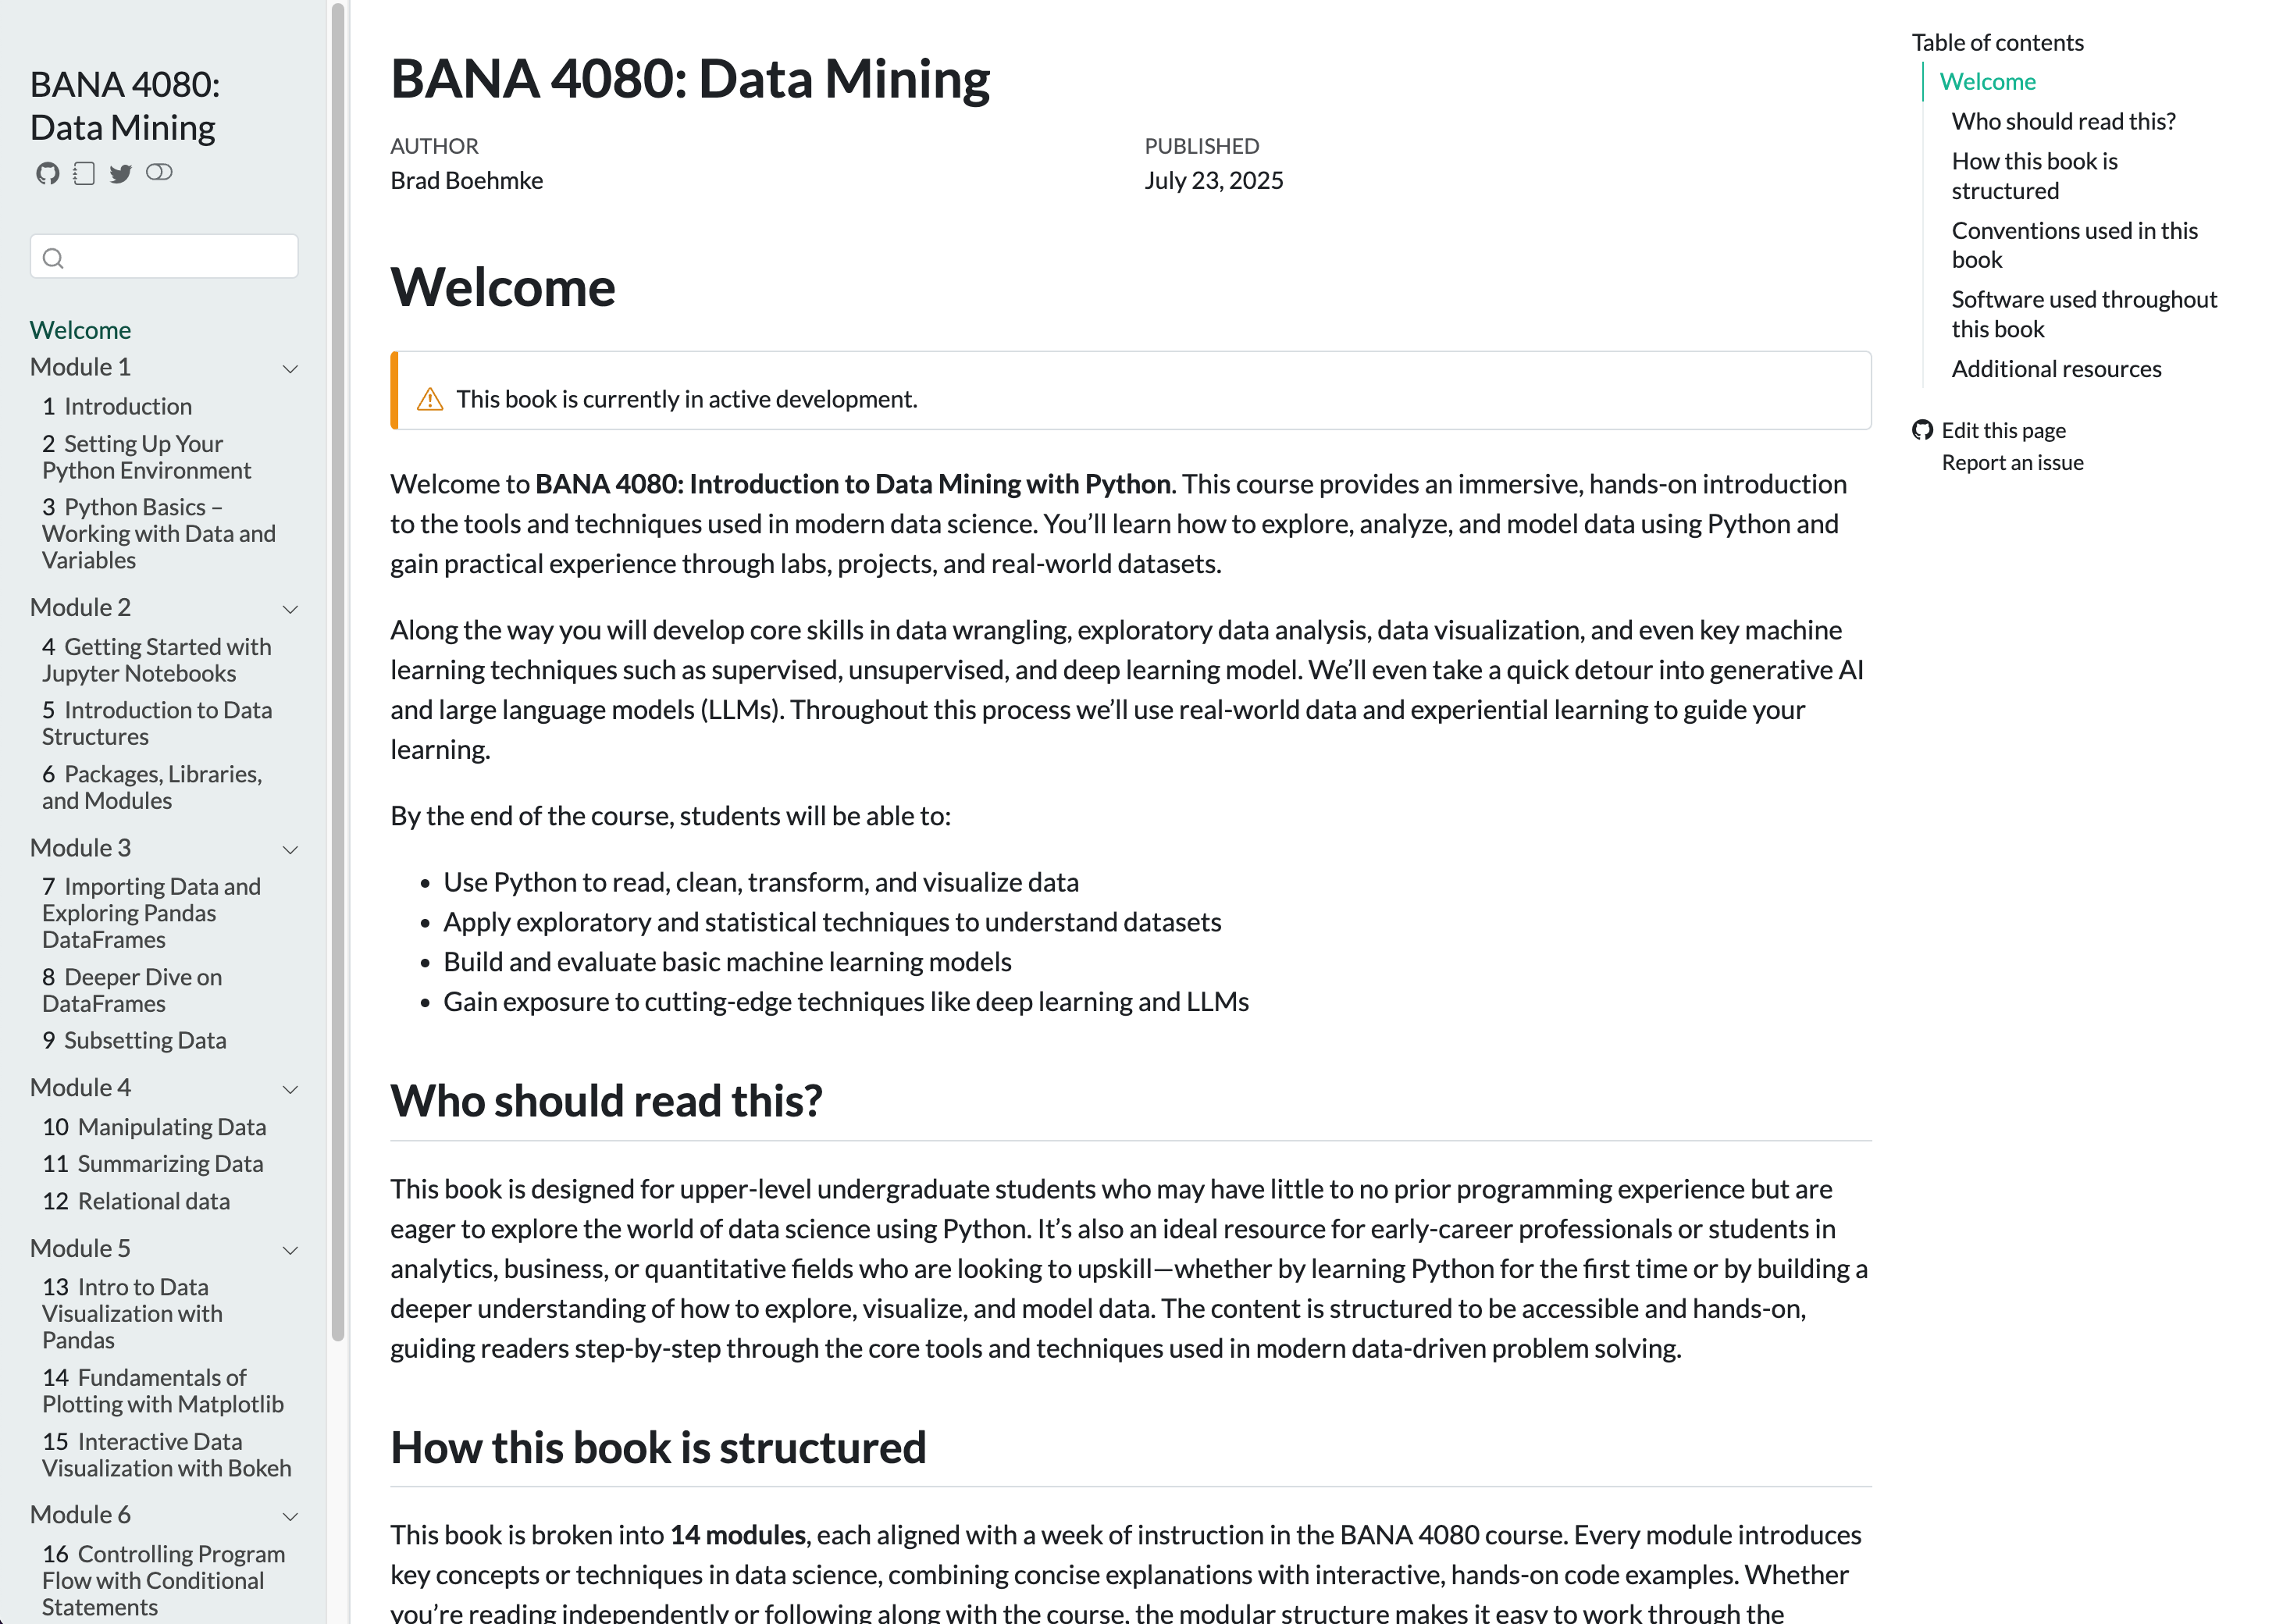
\includegraphics[keepaspectratio]{images/class-book.png}}
\end{center}

Book: \url{https://bradleyboehmke.github.io/uc-bana-4080/}

\subsection{Step 1}\label{step-1}

\begin{tcolorbox}[enhanced jigsaw, leftrule=.75mm, opacityback=0, colback=white, breakable, toprule=.15mm, rightrule=.15mm, left=2mm, colframe=quarto-callout-color-frame, arc=.35mm, bottomrule=.15mm]

Who has read through the {``Start Here!''} module?

\end{tcolorbox}

\pandocbounded{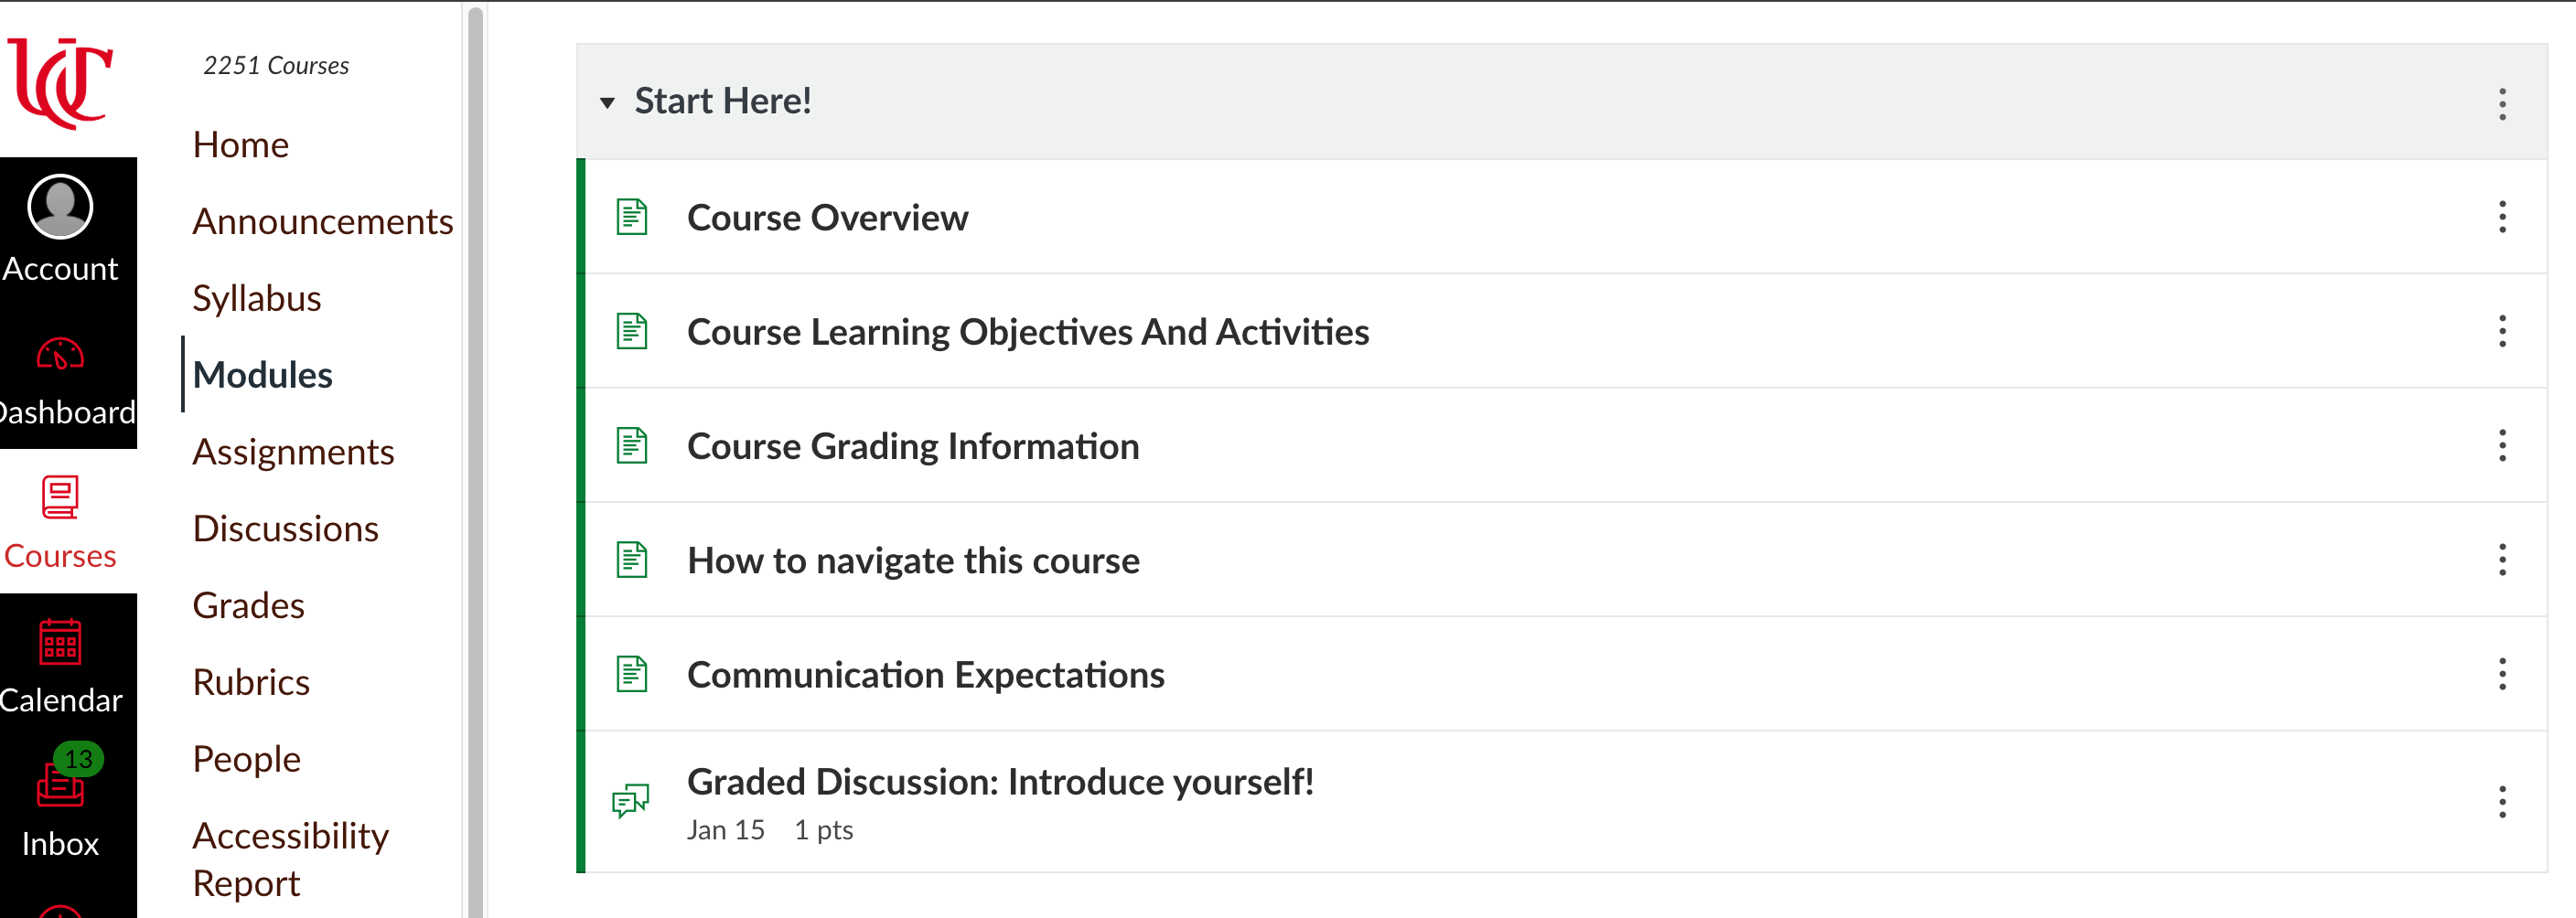
\includegraphics[keepaspectratio]{images/canvas_step1_read_first.png}}

. . .

\begin{tcolorbox}[enhanced jigsaw, leftrule=.75mm, opacityback=0, colback=white, breakable, toprule=.15mm, rightrule=.15mm, left=2mm, colframe=quarto-callout-color-frame, arc=.35mm, bottomrule=.15mm]

Let's hit on a few important items

\end{tcolorbox}

\section{Tools \& Setup Preview}\label{tools-setup-preview}

\subsection{Why Learn to Code? 🤔}\label{why-learn-to-code}

. . .

\begin{itemize}
\tightlist
\item
  Coding = flexibility + power
\item
  Handle real-world data: big, messy, inconsistent
\item
  Automate repetitive tasks
\item
  Think algorithmically and analytically
\end{itemize}

\pandocbounded{\includegraphics[keepaspectratio]{images/learning-to-code.gif}}

\subsection{Why Python? 🤔}\label{why-python}

\begin{itemize}
\tightlist
\item
  Widely used
\item
  Easy-to-read syntax (great for beginners)
\item
  Massive ecosystem: pandas, numpy, matplotlib, scikit-learn
\item
  Community support: tutorials, libraries, AI tools
\item
  \textbf{Most organizations are shifting toward Python} as the primary
  language for their \textbf{data science and engineering codebases}
\end{itemize}

\begin{center}
\includegraphics[width=0.75\linewidth,height=\textheight,keepaspectratio]{images/why-python.gif}
\end{center}

\begin{tcolorbox}[enhanced jigsaw, colbacktitle=quarto-callout-important-color!10!white, opacityback=0, colback=white, opacitybacktitle=0.6, toptitle=1mm, left=2mm, bottomrule=.15mm, breakable, bottomtitle=1mm, rightrule=.15mm, titlerule=0mm, title=\textcolor{quarto-callout-important-color}{\faExclamation}\hspace{0.5em}{Important}, coltitle=black, colframe=quarto-callout-important-color-frame, arc=.35mm, toprule=.15mm, leftrule=.75mm]

Python is the most valuable tool in your analytics toolbox.

\end{tcolorbox}

\subsection{How You'll Run Python: Google
Colab}\label{how-youll-run-python-google-colab}

\paragraph{What is Colab?}\label{what-is-colab}

\begin{itemize}
\tightlist
\item
  💻 Free cloud-based Python environment from Google
\item
  🚫 No software installation needed to get started
\item
  ✅ Works in your browser -- just click and code
\end{itemize}

\paragraph{Why Colab First?}\label{why-colab-first}

\begin{itemize}
\tightlist
\item
  Easy, consistent experience for everyone on Day 1
\item
  Allows us to focus on learning --- not debugging installs
\item
  We'll gradually move toward installing tools locally (e.g., Anaconda,
  Jupyter, VS Code)
\end{itemize}

\pandocbounded{
\includegraphics[keepaspectratio]{images/Google_Colaboratory_SVG_Logo.svg.png}}

\begin{tcolorbox}[enhanced jigsaw, colbacktitle=quarto-callout-important-color!10!white, opacityback=0, colback=white, opacitybacktitle=0.6, toptitle=1mm, left=2mm, bottomrule=.15mm, breakable, bottomtitle=1mm, rightrule=.15mm, titlerule=0mm, title=\textcolor{quarto-callout-important-color}{\faExclamation}\hspace{0.5em}{Important}, coltitle=black, colframe=quarto-callout-important-color-frame, arc=.35mm, toprule=.15mm, leftrule=.75mm]

You'll be up and coding on Day 1 --- no setup headaches!

\end{tcolorbox}

\section{Next Steps}\label{next-steps}

\subsection{Next Steps}\label{next-steps-1}

\begin{enumerate}
\def\labelenumi{\arabic{enumi}.}
\tightlist
\item
  Read the ``Start Here!'' module
\item
  Start working through Module 1's readings
\item
  Be ready to code in Colab on Thursday
\item
  Complete reading quizzes by EOW
\end{enumerate}

\pandocbounded{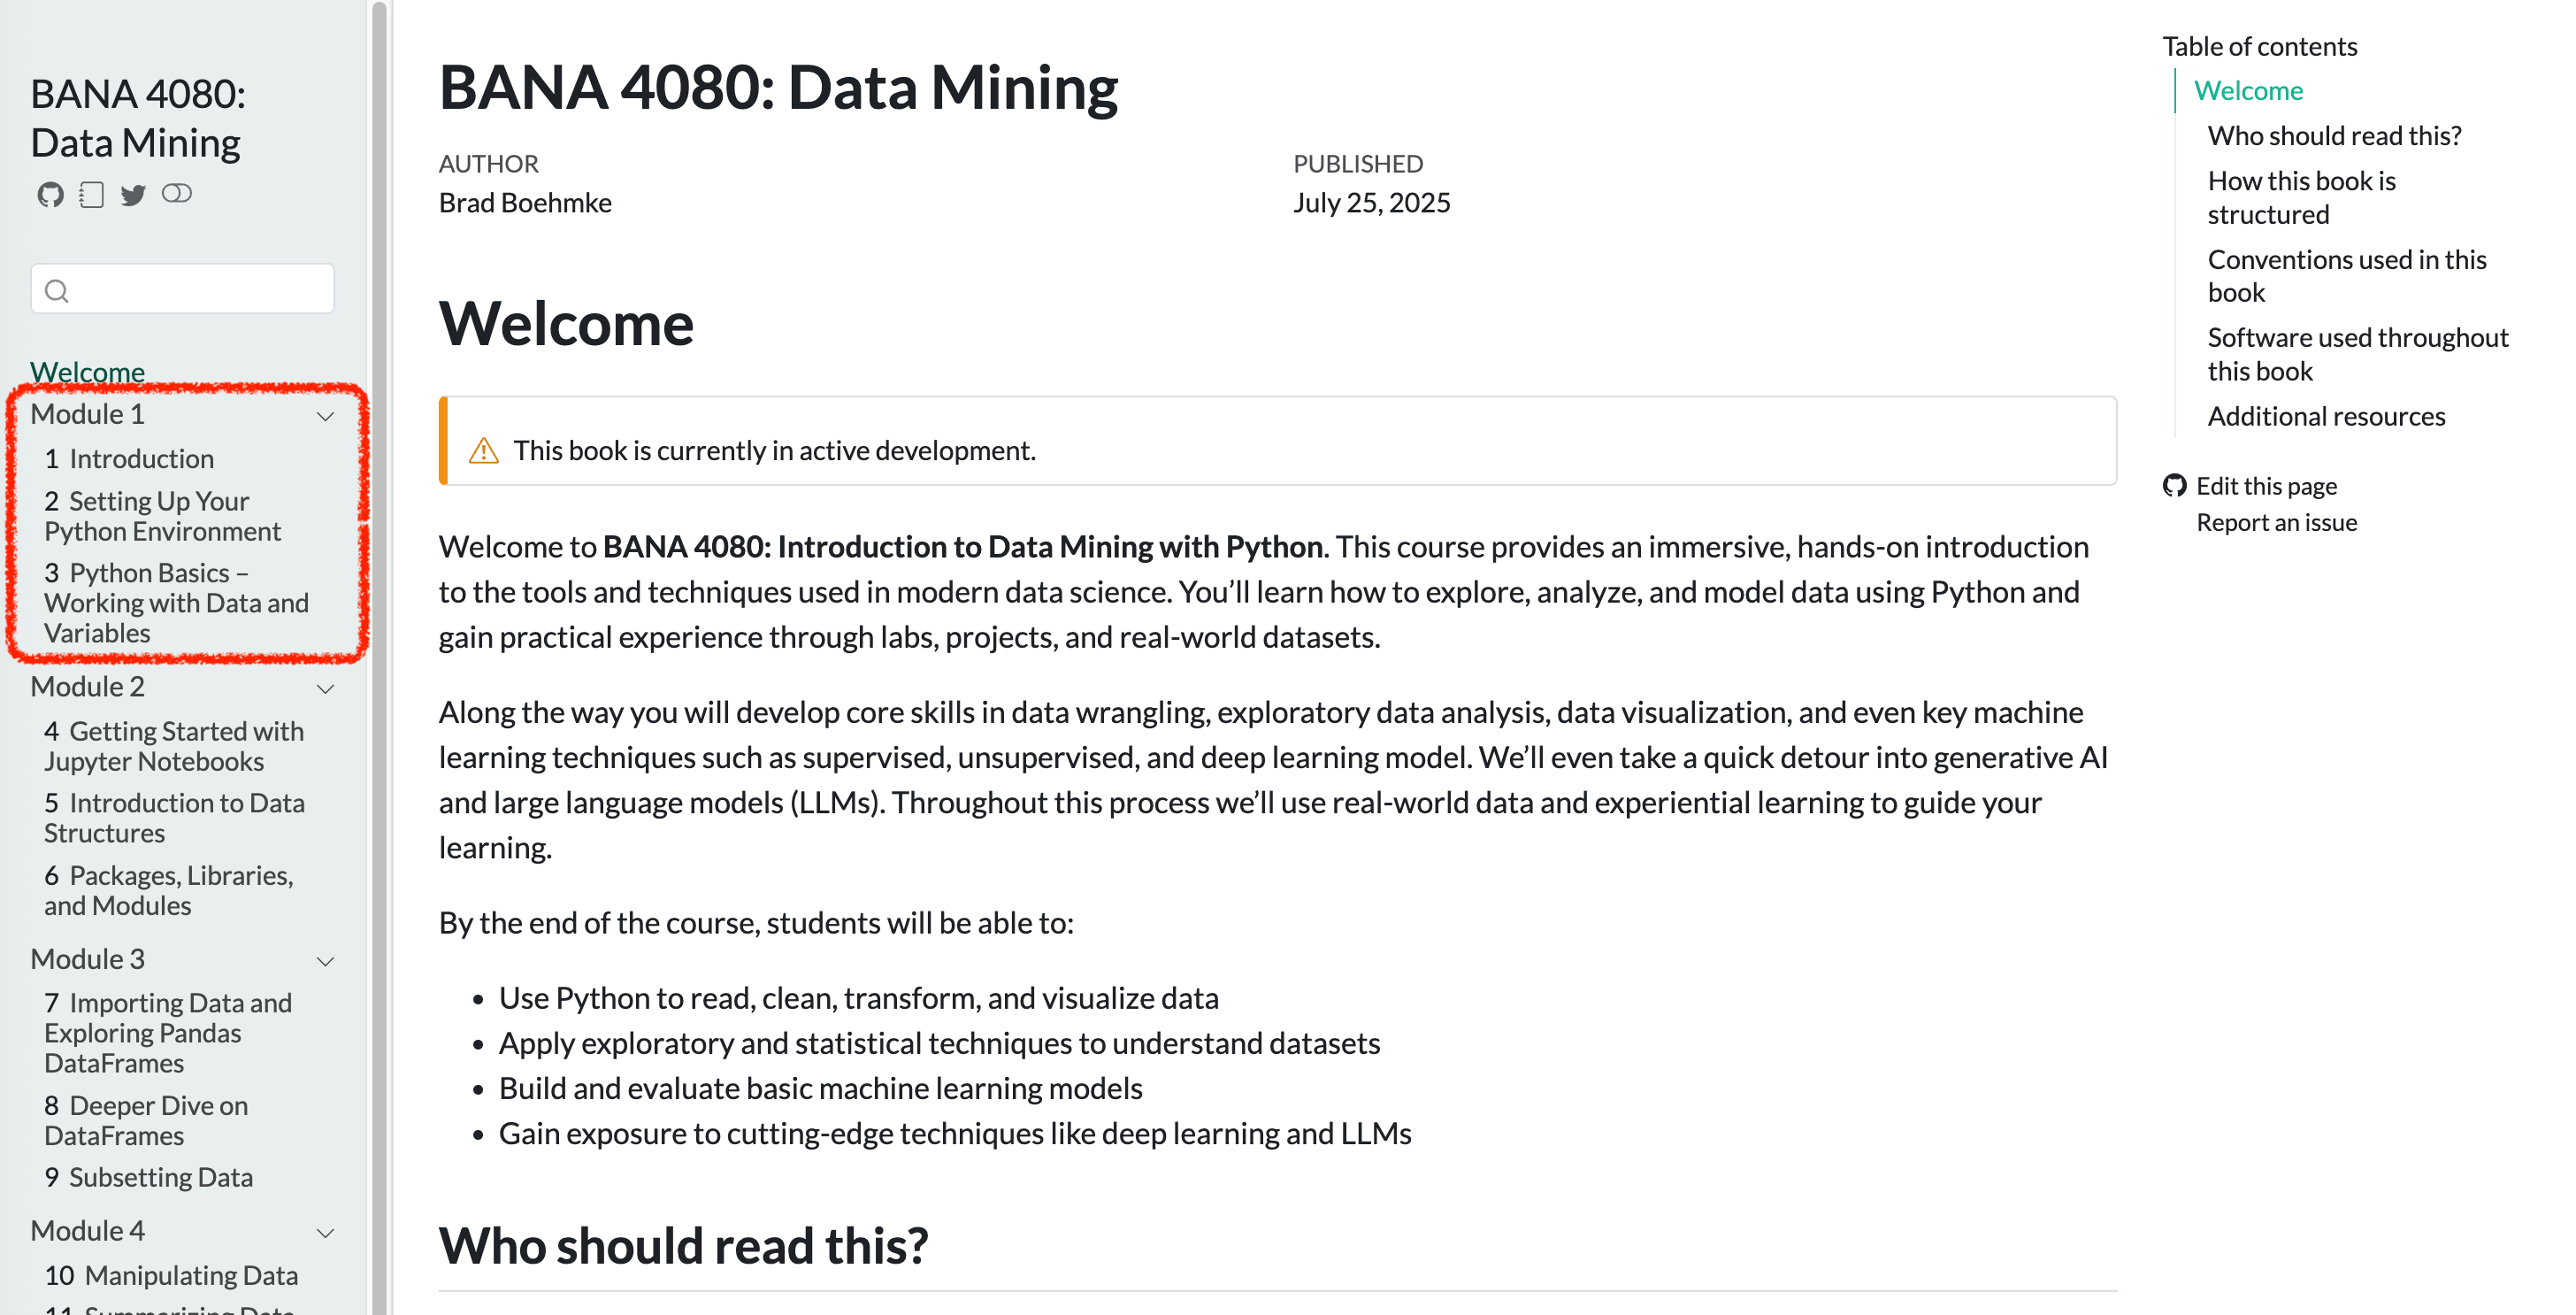
\includegraphics[keepaspectratio]{images/whats-next.png}}

\section{Q\&A}\label{qa}

\subsection{Q\&A 🙋‍♀️}\label{qa-1}

\begin{itemize}
\tightlist
\item
  Open floor for any questions regarding the course structure,
  expectations, or content.
\item
  Discussion on how this course aligns with your academic and career
  goals.
\item
  Or anything else\ldots golf?
\end{itemize}




\end{document}
